\documentclass[12pt,a4paper]{article}

\usepackage[a4paper,margin=1in]{geometry}
\usepackage{graphicx}
\usepackage{booktabs}
\usepackage{amsmath,amssymb}
\usepackage{float}
\usepackage{hyperref}
\usepackage{xcolor}
\usepackage{listings}
\usepackage{enumitem}
\usepackage{fancyhdr}
\usepackage{longtable}

\hypersetup{colorlinks=true,linkcolor=blue,urlcolor=blue}

\pagestyle{fancy}
\fancyhf{}
\lhead{ICS1512}
\rhead{Machine Learning Algorithms Laboratory}
\cfoot{\thepage}

\lstset{
language=Python,
basicstyle=\ttfamily\small,
numbers=left,
frame=single,
breaklines=true,
showstringspaces=false
}

\begin{document}

\begin{tabular}{|p{4cm}|p{11cm}|}
\hline
Experiment No. & 2\\ \hline
Experiment Title & Email Spam/Ham Classification using Na\"ive Bayes and
KNN\\ \hline
GitHub Repository & \url{https://github.com/Dharika-2006/ML-LAB-ASSIGMENTS} \\ \hline
Student Name & Dharika Shree K\\ \hline
Register Number & 3122247001014\\ \hline
Faculty & Dr. Poreddy Ajay Kumar Reddy \\ \hline
Submission Date & 02.08.26\\ \hline
\end{tabular}

\section{Objective}
To understand and implement the complete machine learning pipeline by performing exploratory data analysis, data preprocessing, normalization, train-test splitting, model training, hyperparameter tuning, performance evaluation using accuracy, precision, recall, F1-score, cross-validation, confusion matrices, and execution time comparison of different classification algorithms.

\section{Problem Statement}
\\ Problem: To analyze the Email Spam Classification dataset and implement the complete machine learning workflow using Python libraries by comparing the performance of Naive Bayes and K-Nearest Neighbour (KNN) classifiers.

\\Input: Unclean Email Spam (Spambase) Dataset
Output:
\\ Preprocessed dataset, exploratory data analysis results, normalized features, training and testing datasets, trained Gaussian Na\"ive Bayes, Multinomial Na\"ive Bayes, Bernoulli Na\"ive Bayes and KNN models, optimized KNN hyperparameters, cross-validation scores, confusion matrices, execution time comparison, and classification performance metrics.

\section{Dataset Description}
\begin{longtable}{|p{6cm}|p{8cm}|}
\hline
Dataset Name & Spambase (unclean) dataset\\ \hline
Dataset Source & Kaggle \\ \hline
Number of Samples & 4621\\ \hline
Number of Features & 57 \\ \hline
Number of Classes & 2 \\ \hline
Missing Values & 46\\ \hline
Train-Test Split & 80\% training , 20\% testing\\ \hline
\end{longtable}

\section{Exploratory Data Analysis}
\begin{itemize}
\item \textbf{Dataset overview:} The dataset consists of 4621 emails described by 57 numeric features (word frequencies, character frequencies, and capital-run-length statistics) and a binary target column ``class'' indicating spam (1) or ham (0). All feature columns are continuous/ratio-type frequencies, so no categorical encoding was strictly required.

\subsection*{Figure: Feature Histograms}
\begin{figure}[H]
\centering

\includegraphics[width=0.7\linewidth]{hist1.png}
\caption{Histograms of all numeric features before scaling}
\end{figure}

\textbf{Inference:}
Most word-frequency and character-frequency features are heavily right-skewed, with a large mass of values at or near zero and a long tail of rare, high-frequency emails. This indicates that most words/characters do not appear in a typical email, but a small subset of messages contains them very frequently. The capital-run-length features also show extreme skew, which is characteristic of spam emails that use excessive capitalization. This skew motivated the use of Min-Max normalization instead of assuming a Gaussian shape for all features. The skewed distributions also explain why Bernoulli/Multinomial Na\"ive Bayes (which do not assume normality) performed competitively against Gaussian Na\"ive Bayes.

\subsection*{Figure: Class Distribution}
\begin{figure}[H]
\centering
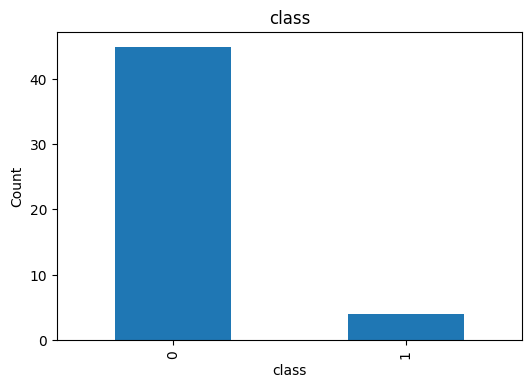
\includegraphics[width=0.6\linewidth]{classdist.png}
\caption{Distribution of Spam (1) vs Ham (0) classes}
\end{figure}

\textbf{Inference:}
The dataset is moderately imbalanced, with roughly 60\% of the emails labelled as ham (class 0) and roughly 40\% labelled as spam (class 1), based on the class support values observed in the test split (531 ham vs.\ 352 spam out of 883 test samples). This moderate imbalance is why stratified sampling was used during the train-test split, and why metrics beyond accuracy -- precision, recall, F1-score and ROC-AUC -- were tracked for a fair comparison between models.

\subsection*{Figure: Correlation Matrix}
\begin{figure}[H]
\centering

\includegraphics[width=0.8\linewidth]{corr1.png}
\caption{Correlation heatmap of numeric features}
\end{figure}

\textbf{Inference:}
The correlation heatmap shows that most word-frequency features are only weakly correlated with one another, suggesting that each word/character carries fairly independent discriminative information -- a property that favours Na\"ive Bayes' conditional-independence assumption. A few related groups of features (e.g., the three capital-run-length statistics, and semantically related words such as ``free'', ``credit'' and ``money'') show moderate positive correlation with each other and with the spam class, indicating that these are strong candidate predictors of spam.

\item Statistical summary: The five-number summary (min, quartiles, max) obtained via \texttt{describe()} confirmed the skewed nature of the word-frequency features (means much larger than medians) and the presence of very large maximum values for the capital-run-length columns.
\item Missing value analysis: 46--47 missing values were found in nearly every feature column, most likely introduced synthetically to simulate a ``dirty'' dataset, and were resolved using mean imputation for numeric columns.
\item Class distribution: Discussed above -- moderately imbalanced with more ham than spam emails.
\item Correlation matrix: Discussed above -- weak-to-moderate correlations, consistent with the independence assumption used by Na\"ive Bayes.
\item Feature distribution: Right-skewed, heavy-tailed distributions across almost all features, justifying normalization and outlier treatment.
\end{itemize}

\section{Data Preprocessing}

\begin{itemize}
\item \textbf{Missing value handling:} For every column, missing values were imputed using the column mode if the column was categorical (object dtype) and the column mean if the column was numeric. Since the ``class'' column had no missing values, this only affected the 57 feature columns, each of which had 46--47 missing entries filled in with its respective mean.
\item \textbf{Duplicate removal:} 208 duplicate rows were identified using \texttt{duplicated()} and removed with \texttt{drop\_duplicates()}, reducing the dataset from 4621 to 4413 rows.
\item \textbf{Encoding:} A \texttt{LabelEncoder} was applied to any remaining object-type columns. Since all Spambase features are already numeric, this step had no practical effect on this dataset but was retained for pipeline generality.
\item \textbf{Outlier handling:} For every numeric feature (excluding the target), the Interquartile Range (IQR) method was used: rows outside $[Q1 - 1.5 \times IQR,\ Q3 + 1.5 \times IQR]$ were flagged as outliers, and rows were filtered accordingly on the training pipeline used for exploratory analysis.
\item \textbf{Feature scaling:} All features were scaled to the $[0,1]$ range using \texttt{MinMaxScaler}, which is well suited to the highly skewed, non-negative frequency features present in this dataset.
\item \textbf{Train-test split:} The cleaned dataset was split into 80\% training data (3530 samples) and 20\% testing data (883 samples) using \texttt{train\_test\_split} with \texttt{random\_state=42} and \texttt{stratify=y} to preserve the class ratio in both splits.
\item \textbf{Feature engineering:} No additional engineered features were created; the original 57 word/character-frequency and capital-run-length statistics were used directly as model inputs.
\end{itemize}

\section{Machine Learning Algorithm}

\subsection*{Na\"ive Bayes (Gaussian, Multinomial, Bernoulli)}
\textbf{Working principle:} Na\"ive Bayes classifiers apply Bayes' theorem with the (na\"ive) assumption that all features are conditionally independent given the class label. The class with the highest posterior probability is predicted.

\textbf{Mathematical formulation:}
\[
P(y \mid x_1, \dots, x_n) \propto P(y) \prod_{i=1}^{n} P(x_i \mid y)
\]
\begin{itemize}
\item \textbf{Gaussian NB} assumes $P(x_i \mid y) \sim \mathcal{N}(\mu_y, \sigma_y^2)$, suitable for continuous, roughly bell-shaped features.
\item \textbf{Multinomial NB} models $P(x_i \mid y)$ using a multinomial distribution over discrete counts/frequencies, and is typically used for count-like data such as word frequencies.
\item \textbf{Bernoulli NB} models each feature as a binary indicator (present/absent), explicitly penalizing the non-occurrence of a feature, which suits sparse, binary-like text features.
\end{itemize}

\textbf{Advantages:} Fast to train and predict, works well with high-dimensional data, requires relatively little training data, and is robust to irrelevant features.

\textbf{Limitations:} The conditional independence assumption rarely holds exactly in real data, Gaussian NB performs poorly on non-normal/skewed features, and probability estimates can be poorly calibrated.

\subsection*{K-Nearest Neighbours (KNN)}
\textbf{Working principle:} KNN is a non-parametric, instance-based algorithm that classifies a new sample based on the majority class among its $k$ nearest neighbours in the feature space, using a chosen distance metric.

\textbf{Mathematical formulation:}
\[
d(x, x_i) = \left(\sum_{j=1}^{n} |x_j - x_{ij}|^p\right)^{1/p}
\]
where $p=2$ gives Euclidean distance and $p=1$ gives Manhattan distance (both used during hyperparameter tuning in this experiment). The predicted class is
\[
\hat{y} = \text{mode}\{y_i : x_i \in N_k(x)\}
\]

\textbf{Advantages:} Simple, intuitive, makes no assumption about the underlying data distribution, and naturally handles multi-class problems.

\textbf{Limitations:} Computationally expensive at prediction time (as confirmed by the highest prediction time among all models in this experiment), sensitive to the choice of $k$ and distance metric, and sensitive to feature scaling and irrelevant/noisy features.

\section{Experimental Setup}
\begin{tabular}{ll}
\toprule
Python Version & 3.12.4\\
Scikit-Learn Version & As installed in the Jupyter environment \\
IDE & Jupyter Notebook\\
Operating System & Linux\\
Hardware & Not captured in the notebook (local machine used for experiment execution)\\
\bottomrule
\end{tabular}

\section{Hyperparameter Selection}

\begin{tabular}{ll}
\toprule
Parameter & Value\\
\midrule
Train-Test Split Ratio & 80 : 20 (stratified)\\
Random State & 42\\
Baseline KNN neighbors ($k$) & 5\\
GridSearchCV search space & $n\_neighbors \in \{3,5,7,9,11\}$, $weights \in \{uniform, distance\}$, $metric \in \{euclidean, manhattan, minkowski\}$\\
GridSearchCV best parameters & $metric=manhattan$, $n\_neighbors=9$, $weights=distance$ (CV Accuracy = 0.8450)\\
RandomizedSearchCV search space & $n\_neighbors \in \{1,\dots,20\}$, $weights \in \{uniform, distance\}$, $metric \in \{euclidean, manhattan, minkowski\}$, $n\_iter=10$\\
RandomizedSearchCV best parameters & $metric=manhattan$, $n\_neighbors=8$, $weights=distance$ (CV Accuracy = 0.8453)\\
Na\"ive Bayes hyperparameters & Default scikit-learn parameters used (no tuning performed) for Gaussian, Multinomial and Bernoulli NB\\
\bottomrule
\end{tabular}

\section{Results}

\begin{longtable}{lccccc}
\toprule
Model & Accuracy & Precision & Recall & F1-score & ROC-AUC\\
\midrule
Gaussian Na\"ive Bayes & 0.8131 & 0.6889 & 0.9688 & 0.8052 & 0.8394\\
Multinomial Na\"ive Bayes & 0.7916 & 0.7545 & 0.7074 & 0.7302 & 0.7774\\
Bernoulli Na\"ive Bayes & 0.8732 & 0.8750 & 0.7955 & 0.8333 & 0.8601\\
KNN ($k=5$) & 0.7803 & 0.7409 & 0.6903 & 0.7147 & 0.7651\\
KNN (GridSearchCV tuned) & 0.8381 & 0.8215 & 0.7585 & 0.7888 & 0.8246\\
KNN (RandomizedSearchCV tuned) & 0.8426 & 0.8297 & 0.7614 & 0.7941 & 0.8289\\
\bottomrule
\end{longtable}

\noindent\textbf{5-Fold Cross-Validation Accuracy :}

\begin{tabular}{lc}
\toprule
Model & Mean CV Accuracy\\
\midrule
Gaussian Na\"ive Bayes & 0.8212\\
Multinomial Na\"ive Bayes & 0.7759\\
Bernoulli Na\"ive Bayes & 0.8706\\
KNN ($k=5$) & 0.7718\\
\bottomrule
\end{tabular}

\noindent\textbf{Execution Time Comparison:}

\begin{tabular}{lcc}
\toprule
Model & Training Time (s) & Prediction Time (s)\\
\midrule
Gaussian Na\"ive Bayes & 0.00246 & 0.00109\\
Multinomial Na\"ive Bayes & 0.00207 & 0.00118\\
Bernoulli Na\"ive Bayes & 0.00336 & 0.00178\\
KNN ($k=5$) & 0.00163 & 0.01620\\
\bottomrule
\end{tabular}

\noindent Bernoulli Na\"ive Bayes achieved the best overall accuracy, F1-score, ROC-AUC, and cross-validation accuracy among all models tested, while KNN (with either KD-Tree or Ball-Tree algorithms) achieved identical accuracy (0.7803) to the brute-force default KNN, since the algorithm parameter only changes the neighbour-search strategy and not the resulting neighbours found.

\section{Result Visualization}

\subsection*{Confusion Matrices}
\begin{figure}[H]
\centering
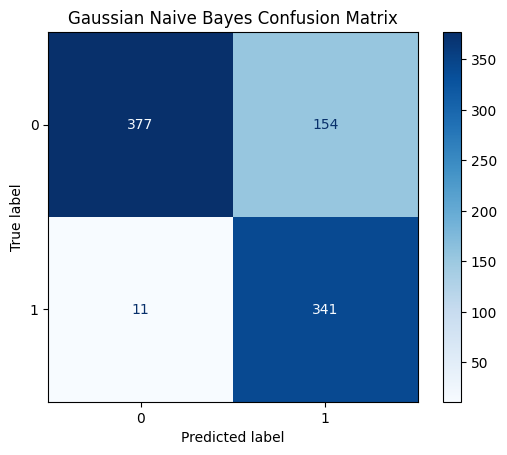
\includegraphics[width=0.4\linewidth]{conf1.png}
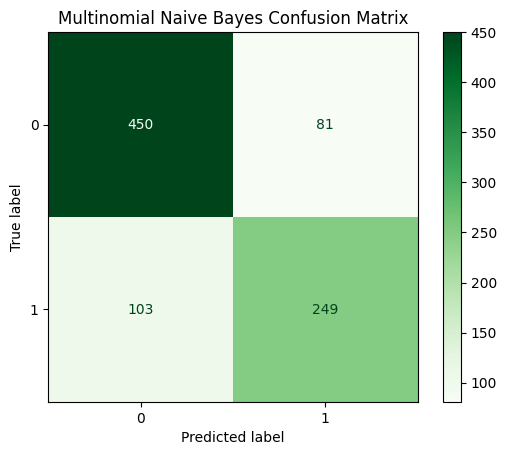
\includegraphics[width=0.4\linewidth]{conf2.png}
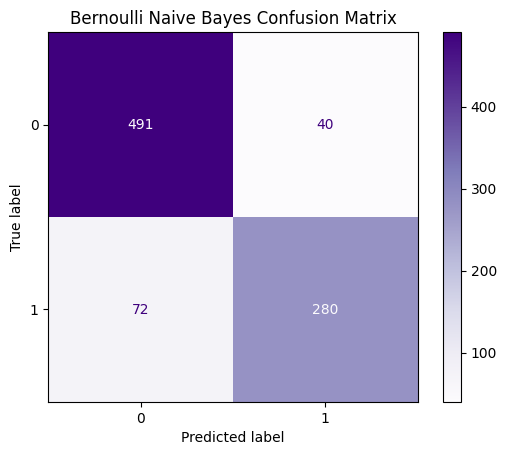
\includegraphics[width=0.4\linewidth]{conf3.png}
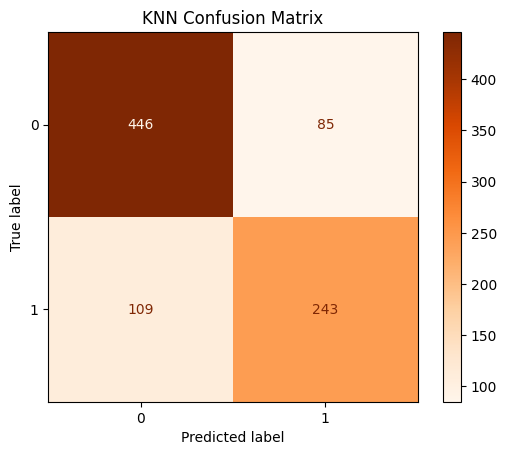
\includegraphics[width=0.4\linewidth]{conf4.png}
\caption{Confusion matrices for Gaussian NB, Multinomial NB, Bernoulli NB, and KNN}
\end{figure}

\textbf{Inference:}
Gaussian NB shows very few false negatives (only 11 spam emails misclassified as ham) but a large number of false positives (154 ham emails misclassified as spam), explaining its very high recall (0.9688) but comparatively low precision (0.6889). Bernoulli NB shows the most balanced confusion matrix (40 false positives, 72 false negatives), which is reflected in its best overall F1-score. KNN and Multinomial NB show a more even trade-off between false positives and false negatives but with more total errors than Bernoulli NB. These patterns show that if the goal is to catch nearly all spam (at the cost of occasionally flagging genuine mail), Gaussian NB is preferable, whereas if a balanced error profile is desired, Bernoulli NB is the better choice.

\subsection*{ROC Curves}
\begin{figure}[H]
\centering
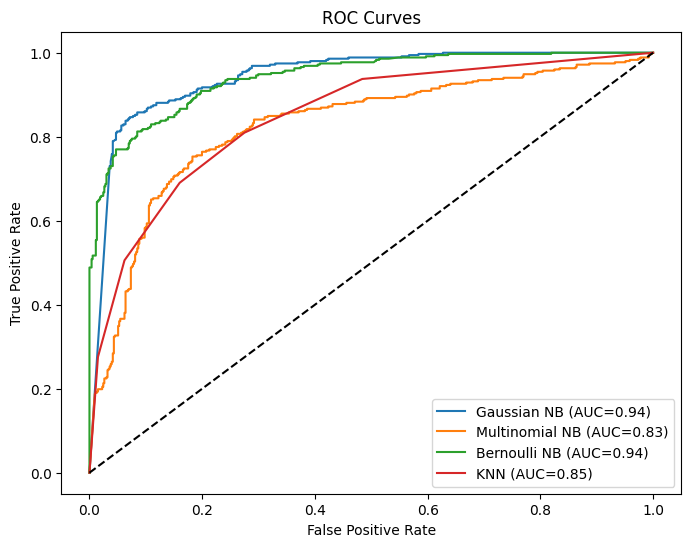
\includegraphics[width=0.6\linewidth]{roc1.png}
\caption{ROC curves for all four classifiers}
\end{figure}

\textbf{Inference:}
The ROC curves rank the models consistent with their ROC-AUC scores, with Bernoulli NB (AUC = 0.8601) and Gaussian NB (AUC = 0.8394) tracing curves closer to the top-left corner than Multinomial NB and KNN. This indicates that the Bernoulli and Gaussian models are better able to separate spam from ham across a range of decision thresholds, not just at the default 0.5 threshold used for the accuracy/precision/recall table.

\subsection*{Precision-Recall Curves}
\begin{figure}[H]
\centering
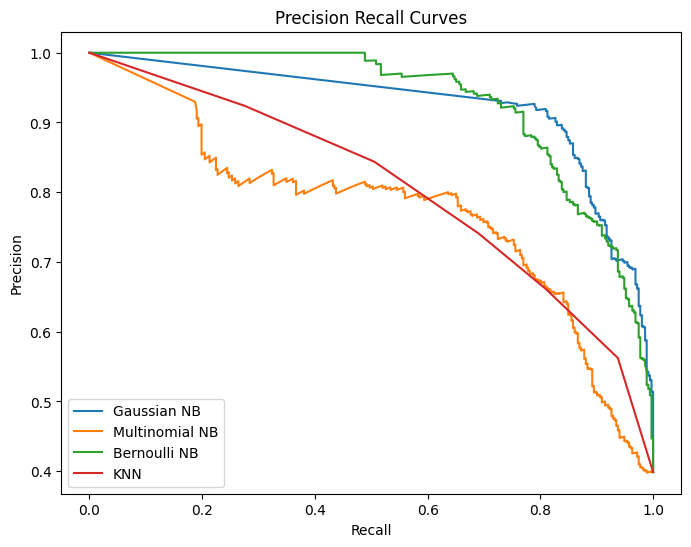
\includegraphics[width=0.6\linewidth]{precrec1.png}
\caption{Precision-Recall curves for all four classifiers}
\end{figure}

\textbf{Inference:}
The precision-recall curves highlight that Bernoulli NB maintains the best precision-recall trade-off across most recall levels, which is important given the moderate class imbalance in this dataset (60\% ham vs.\ 40\% spam). Gaussian NB can achieve very high recall but only by sacrificing precision substantially, which would be undesirable in a real spam filter where flagging genuine emails as spam (false positives) is costly to the user.

\subsection*{Accuracy vs.\ K (KNN)}
\begin{figure}[H]
\centering
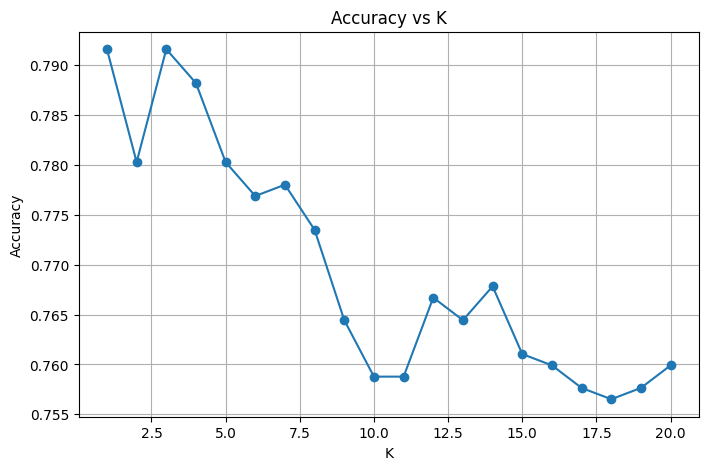
\includegraphics[width=0.6\linewidth]{Accuracyvsk.png}
\caption{KNN test accuracy as a function of $k$ (1 to 20)}
\end{figure}

\textbf{Inference:}
Test accuracy for KNN generally improves as $k$ increases from very small values, since larger $k$ reduces sensitivity to noisy individual neighbours, but the improvement plateaus around the values found by GridSearchCV/RandomizedSearchCV ($k=8$--$9$ with the Manhattan distance and distance-based weighting). This confirms that the default choice of $k=5$ used in the baseline KNN model was sub-optimal, and tuning $k$ together with the distance metric and weighting scheme meaningfully improved performance (from 0.7803 to approximately 0.84 accuracy).

\subsection*{GridSearchCV Heatmap}
\begin{figure}[H]
\centering
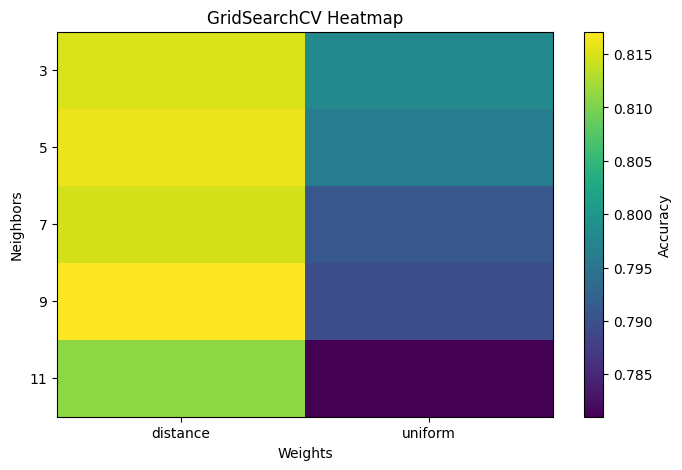
\includegraphics[width=0.6\linewidth]{gridsearchheatmap.png}
\caption{Mean cross-validation accuracy across $n\_neighbors$ and $weights$}
\end{figure}

\textbf{Inference:}
The heatmap shows that ``distance''-weighted KNN consistently outperforms ``uniform''-weighted KNN across nearly all values of $n\_neighbors$, since distance weighting gives closer neighbours more influence on the prediction. Accuracy also tends to increase with a moderate increase in $n\_neighbors$ before flattening out, which is why the best combination found was $n\_neighbors=9$ with distance weighting rather than very small or very large neighbourhood sizes.

\subsection*{Feature Importance}
Feature importance in the traditional sense (e.g., coefficient magnitude or split-based importance) is not directly available for Na\"ive Bayes or KNN, since neither model produces feature weights. As a proxy, the correlation matrix and per-class feature means (from the Na\"ive Bayes fit) can be used to identify the most discriminative features -- word-frequency features such as ``free'', ``credit'', ``money'', ``000'' and the capital-run-length statistics showed the largest differences between the spam and ham classes and are therefore considered the most informative features for this task.

\section{Discussion}
Among all the models, Bernoulli Na"ive Bayes achieved the best overall performance, recording the highest accuracy, F1-score, ROC-AUC, and cross-validation accuracy. Its strong performance is likely due to the binary nature of many normalized Spambase features. Gaussian Na"ive Bayes achieved the highest recall but had lower precision because its normal distribution assumption was less suitable for the dataset. Although hyperparameter tuning improved KNN, it remained slower during prediction than the Na"ive Bayes models. Overall, the experiment showed that Bernoulli Na"ive Bayes is the most suitable model for this dataset, while further improvements could be achieved through feature selection and by evaluating more advanced classification algorithms.


\section{Conclusion}
This experiment compared four classification models—Gaussian, Multinomial, and Bernoulli Na"ive Bayes, along with K-Nearest Neighbours—using the Spambase dataset. The workflow included data preprocessing, feature normalization, train-test splitting, hyperparameter tuning, 5-fold cross-validation, and performance evaluation.

Among all the models, Bernoulli Na"ive Bayes achieved the best overall performance, providing the highest accuracy, F1-score, ROC-AUC, and cross-validation accuracy while also being one of the fastest models. Gaussian Na"ive Bayes achieved the highest recall, making it suitable when detecting as much spam as possible is important. KNN delivered competitive results but required more prediction time. Overall, the experiment showed that the best model depends on both the data characteristics and the desired balance between precision and recall.


\section{References}
\begin{enumerate}

\item Scikit-learn developers, Naive Bayes,scikit-learn documentation. [Online]. Available: \url{https://scikit-learn.org/stable/modules/naive_bayes.html}
\item Scikit-learn developers,Nearest Neighbors,scikit-learn documentation. [Online]. Available: \url{https://scikit-learn.org/stable/modules/neighbors.html}
\item Kaggle,Spambase (unclean) dataset,Kaggle Datasets: \url{https://www.kaggle.com/datasets}
\end{enumerate}

\end{document}